
%!TEX program = xelatex
\documentclass[letterpaper,12pt]{exam}
\usepackage{../videoNotes}
\usepackage{xcolor}
\usepackage[dvipsnames]{xcolor}
\usepackage{soul}

\newcommand{\unit}{Unit 01}
\pagestyle{headandfoot}
\firstpageheader{CSC 264 \semester\ \  \unit}{}{Name: $\rule{6cm}{0.15mm}$}
\runningheader{CSC 264 \semester}{\unit}{Page \thepage\ of \numpages}
\firstpagefooter{}{}{}
\runningfooter{}{}{}

\begin{document}



\section*{\unit\_000 -- Arithmetic and Data Representation} 
\par{\fontfamily{qzc}\selectfont\textbf{Video Length 4:16 }}
\begin{questions}

\begin{samepage}
    \question Will you be able to use a calculator on the exams?
    \vspace{5mm}
\end{samepage}
\par
 

 \begin{samepage} 
     \question Using the cheatsheet, What is $ 16 x 12 $ ? \rule{2cm}{0.15mm}     \vspace{5mm}
 \end{samepage}
 \par
 \begin{samepage}
     \question Do you anticipate a problem with not being able to use a calculator on the exam?  If so, I will see if we can work together to figure out a solution.
     \vspace{5mm}
 \end{samepage}
 \par
   
----------------------------------
\section*{\unit\_010 -- Decimal }
\par{\fontfamily{qzc}\selectfont\textbf{Video Length 10:15}}
\begin{samepage}
    \question What is any number raised to the zero power?
    \vspace{5mm}
\end{samepage}
ar
\rule{0.5\textwidth}{.4pt} %End of section

\begin{samepage}
    \question What is any number raised to the first power?
    \vspace{5mm}
\end{samepage}
\par
 

\begin{samepage}
    \question Why doesn't the base ten number system have a symbol for ten?
    \vspace{5mm}
\end{samepage}
\par
 
\begin{samepage}
    \question What number follows 999 in base ten?
    \vspace{5mm}
\end{samepage}
\par
 
----------------------------------

\section*{\unit\_020 -- Base 5}
\par{\fontfamily{qzc}\selectfont\textbf{Video Length 4:45}}

Note:  Base 5 will not be on the exam.  The point of this video is to explain the system and how it applies to other bases.

The video is for base 5, but I will ask the following questions for base 3.  If you understand the system, you should be able to apply the ideas to base 3.

\begin{samepage}
    \question What are the symbols used in base 3?
    \vspace{5mm}
\end{samepage}
\begin{samepage}
    \question How would three be represented in base 3?
    \vspace{5mm}
\end{samepage}
ar

\begin{samepage}
    \question What is $3^2$ in base 10?
    \vspace{5mm}
\end{samepage}
\par

\begin{samepage}
    \question How would four be represented in base 3?
    \vspace{5mm}
\end{samepage}

\begin{samepage}
    \question Count to fifteen in base 3.
    \vspace{25mm}
\end{samepage}
\par
 
\begin{samepage}
    \question What is $211_3$ in base 10?
    \vspace{5mm}
\end{samepage}
\par

\rule{0.5\textwidth}{.4pt} %End of section
%----------------------------------

\section*{\unit\_030 -- Base 2 (Binary) }
\par{\fontfamily{qzc}\selectfont\textbf{Video Length 13:00}}
\begin{samepage}
    \question What is Base 2 called?
    \vspace{5mm}
\end{samepage}
ar

Fill in the following table.  Write the powers of 2 in the second column.

\begin{Large}
\begin{tabular}{| c | c |}

 \hline
    Power of 2& Value \\
    \hline
 $2^0 $ &  \\
 \hline 
$2^1 $ &  \\
 \hline 
$2^2 $ &  \\
 \hline 
$2^3 $ &  \\
 \hline 
$2^4 $ &  \\
 \hline 
$2^5 $ &  \\
 \hline 
$2^6 $ &  \\
 \hline 
$2^7 $ &  \\
 \hline 
$2^8 $ &  \\
 \hline 

\end{tabular}
\end{Large}
\begin{samepage}
    \question How would you represent two in binary?
    \vspace{5mm}
\end{samepage}
\newpage
 
\begin{samepage}
    \question How would you represent three in binary?
    \vspace{5mm}
\end{samepage}

\begin{samepage}
    \question Count to fifteen in binary.
    \par
\begin{huge}
\begin{tabular}{| c | c |}

 \hline
    Decimal& Binary \\
    \hline
 0 &  \hspace{30mm}\\
 \hline 
 1 &  \\
 \hline 
 2 &  \\
 \hline 
 3 &  \\
 \hline 
 4 &  \\
 \hline 
 5  &  \\
 \hline 
 6 &  \\
 \hline 
 7 &  \\
 \hline 
 8  &  \\
 \hline 
 9 &  \\
 \hline 
 10 &  \\
 \hline 
 11 &  \\
 \hline 
 12 &  \\
 \hline 
 13 &  \\
 \hline 
 14  &  \\
 \hline 
 15 &  \\
 \hline 
 
\end{tabular}
\end{huge}

\end{samepage}
\par
 
\begin{samepage}
    \question What is $1011_2$ in base 10?
    \vspace{5mm}
\end{samepage}
\par
\begin{samepage}
    \question What does 0b1111 mean?  (Focus on the 0b)
    \vspace{5mm}
\end{samepage}
\par
 

\rule{0.5\textwidth}{.4pt} %End of section
%----------------------------------

\section*{\unit\_040 -- Base 16 (Hexadecimal) }
\par{\fontfamily{qzc}\selectfont\textbf{Video Length 16:00}}
\begin{samepage}
    \question How would sixteen be written in base 16?
    \vspace{5mm}
\end{samepage}

\begin{samepage}
    \question Write the powers of 16 in the following table.
\par
    \begin{Large}
\begin{tabular}{| c | c |}

 \hline
    Power of 16& Value \\
    \hline
 $16^0 $ &  \\
 \hline 
$16^1 $ &  \\
 \hline 
$16^2 $ &  \\
 \hline 
$16^3 $ &  \\
 \hline 
\end{tabular}
\end{Large}
\end{samepage}

\begin{samepage}
    \question Fill in the columns for hexadecimal and binary.  Write the binary as 4 digits.
 \par
 \begin{large}
    \begin{tabular}{| c | c | c |}
    \hline
        Decimal & Hexadecimal & \ \ \ \ \ \ \ \ \ \ \ Binary\ \ \ \ \ \ \ \ \ \ \ \\
        \hline
    0 & 0 & 0000 \\ 
    1 &  &  \\  
\hline
    2 &  & \  \\ 
    3 &  & \  \\  
\hline
    4 &  & \  \\ 
    5 &  & \  \\  
\hline
    6 &  & \  \\ 
    7 &  & \  \\  
\hline
    8 &  & \  \\ 
    9 &  & \  \\  
\hline
    10 &  & \  \\ 
    11 &  & \  \\  
\hline
    12 &  & \  \\ 
    13 &  & \  \\  
\hline
    14 &  & \  \\ 
    15 &  & \  \\  
\hline
\end{tabular}
\end{large}
\end{samepage}
\par
 
\begin{samepage}
    \question A \rule{2cm}{0.15mm} is a group of 8 bits.  A \rule{3cm}{0.15mm} is a group of 4 bits.
    \vspace{5mm}
\end{samepage}
\par
 
\begin{samepage}
    \question What is $d3_{16}$ in base 10?
    \vspace{5mm}
\end{samepage}


\rule{0.5\textwidth}{.4pt} %End of section
%----------------------------------
\section*{\unit\_050 -- Convert from Decimal}
\par{\fontfamily{qzc}\selectfont\textbf{Video Length 16:16}}
\begin{samepage}
    \question  Convert $42_{10}$ to binary.  Show your work.
    \vspace{25mm}
\end{samepage}
\begin{samepage}
    \question Convert $134_{10}$ to hexadecimal.  Show your work.
    \vspace{25mm}
\end{samepage}
\par
 
\rule{0.5\textwidth}{.4pt} %End of section
%----------------------------------
\section*{\unit\_60 -- Bit Space}
\par{\fontfamily{qzc}\selectfont\textbf{Video Length 10:00}}
\begin{samepage}
    \question If you have 1 bit, how many different values can be stored?
    \vspace{5mm}
\end{samepage}
\begin{samepage}
    \question Suppose you are a secret agent passing messages to your contact.  You have an office with 5 windows.  Each window has curtains that may either be open or closed (they cannot be set to half open).  You give your contact a list of patterns of windows and the meaning of each message.  How many different prearranged messages could you send to your contact using the five windows?
    \vspace{5mm}
\end{samepage}
\par
 \begin{samepage}
     \question What is the general formula for figuring out how many combinations are possible with n bits?
     \vspace{5mm}
 \end{samepage}
 \par
  
\rule{0.5\textwidth}{.4pt} %End of section
%----------------------------------

\section*{\unit\_070 -- Bytes, Words, Double Words, and Quads}
\par{\fontfamily{qzc}\selectfont\textbf{Video Length }}

\begin{samepage}
    \question What is a byte?
    \vspace{5mm}
\end{samepage}
\par
 

\begin{samepage}
    \question Why was Octal important in the past?
    \vspace{5mm}
\end{samepage}

\begin{samepage}
    \question What is the problem with 6-bit computers?
    \vspace{5mm}
\end{samepage}
\par
 \begin{samepage}
     \question Why does standard ASCII code have 127 different values?
     \vspace{5mm}
 \end{samepage}
 \par
 \begin{samepage}
     \question How many bytes are in a word? \rule{2cm}{0.15mm} How many bits? \rule{2cm}{0.15mm}
     \vspace{5mm}
 \end{samepage}
  \begin{samepage}
     \question How many bytes are in a double word? \rule{2cm}{0.15mm} How many bits? \rule{2cm}{0.15mm} How many words? \rule{2cm}{0.15mm}
     \vspace{5mm}
 \end{samepage}
 \begin{samepage}
     \question How many bytes are in a quad? \rule{2cm}{0.15mm} How many bits? \rule{2cm}{0.15mm} How many words? \rule{2cm}{0.15mm}
     \vspace{5mm}
 \end{samepage} 
  
\rule{0.5\textwidth}{.4pt} %End of section
%----------------------------------

\section*{\unit\_080 -- Binary ⇄ Hexadecimal Conversion}
\par{\fontfamily{qzc}\selectfont\textbf{Video Length }}
\begin{samepage}
    \question Do the following conversions.  Do them directly.  Remember to use the cheatsheet if you need it.
    \{\begin{itemize}
      \item  0b1011 1101 = 0x\_\_\_\_\_\_\_\_\_\_\_\_\\
      \item  0b0111 1000 = 0x\_\_\_\_\_\_\_\_\_\_\_\_\\
      \item  0b1111 1111 = 0x\_\_\_\_\_\_\_\_\_\_\_\_\\
      \item  0b000 00000 = 0x\_\_\_\_\_\_\_\_\_\_\_\_
      \item  0x3A = 0b\_\_\_\_\_\_\_\_\_\_\_\_\_\_\_\_\_\_\_\_\_\_\_\_\\
      \item  0x12 = 0b\_\_\_\_\_\_\_\_\_\_\_\_\_\_\_\_\_\_\_\_\_\_\_\_\\
      \item  0xAA = 0b\_\_\_\_\_\_\_\_\_\_\_\_\_\_\_\_\_\_\_\_\_\_\_\_\\
    \end{itemize}
\end{samepage}

\rule{0.5\textwidth}{.4pt} %End of section
%----------------------------------
  %%%%%%%%%%%%%%%%%%%%%%%%%%%%%%%%%%%%%%%%%%%%%%%%%%%%%
\begin{center}
    \rule{0.5\textwidth}{.4pt}
\end{center}
Do you have any questions or concerns? Please write any lingering questions you have here.

%----------------------------------
\end{questions}
%footer
\vfill
\begin{center}
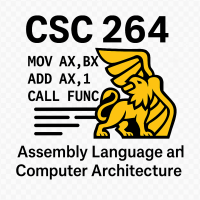
\includegraphics{../csc264Logo}
\end{center}
\end{document} 